\documentclass[tikz,border=6pt]{standalone}
\usepackage{amsmath}
\usetikzlibrary{arrows.meta,positioning,calc,decorations.pathreplacing}
\begin{document}
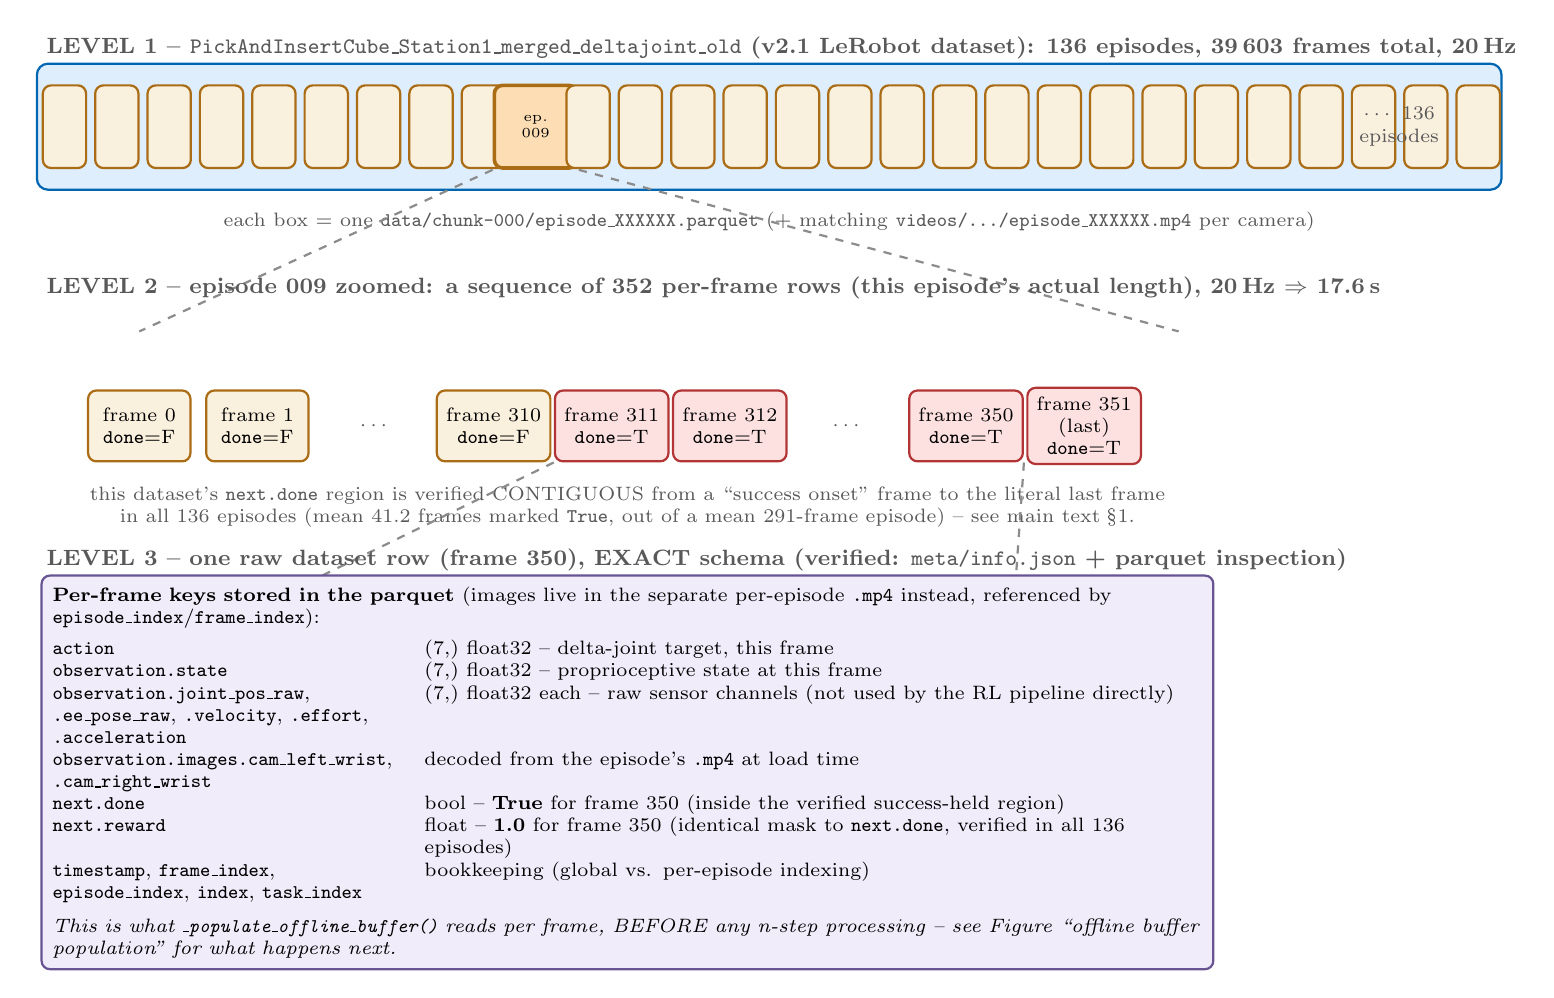
\begin{tikzpicture}[
    >={Latex[length=2.4mm,width=1.7mm]}, font=\small,
    ds/.style={draw=dsline,thick,rounded corners=4pt,fill=dsfill,minimum height=1.6cm},
    ep/.style={draw=epline,thick,rounded corners=3pt,fill=epfill,minimum width=0.55cm,minimum height=1.05cm,align=center,font=\tiny},
    ephi/.style={ep,draw=epline,line width=1.3pt,fill=epfillhi},
    zoomline/.style={draw=black!45,thick,dashed},
    key/.style={draw=keyline,thick,rounded corners=3pt,fill=keyfill,align=left,font=\scriptsize,inner sep=4pt},
    hdr/.style={font=\small\bfseries,text=black!65},
    lbl/.style={font=\scriptsize,align=center,text=black!65},
]
\definecolor{dsline}{RGB}{0,102,178}    \definecolor{dsfill}{RGB}{222,238,252}
\definecolor{epline}{RGB}{170,108,20}   \definecolor{epfill}{RGB}{250,240,222}
\definecolor{epfillhi}{RGB}{253,222,180}
\definecolor{keyline}{RGB}{104,84,146}  \definecolor{keyfill}{RGB}{240,236,250}
\definecolor{doneline}{RGB}{178,52,52}  \definecolor{donefill}{RGB}{253,225,225}

% ================= LEVEL 1: the whole dataset, as a long row of episode boxes =================
\node[hdr] at (0,4.6) [anchor=west] {\footnotesize LEVEL 1 -- \texttt{PickAndInsertCube\_Station1\_merged\_deltajoint\_old} (v2.1 LeRobot dataset): 136 episodes, 39\,603 frames total, 20\,Hz};

\node[ds,minimum width=18.6cm] (dsbox) at (9.3,3.6) {};
\foreach \i in {0,...,27}{
  \pgfmathsetmacro{\w}{0.62+0.08*mod(\i*7,5)}
  \ifnum\i=9
    \node[ephi,minimum width=1.05cm] (epHi) at (0.35+\i*0.665,3.6) {ep.\\009};
  \else
    \node[ep] at (0.35+\i*0.665,3.6) {};
  \fi
}
\node[lbl] at (18.6-1.3,3.6) {$\cdots$ 136\\episodes};
\node[lbl,anchor=north] at (dsbox.south) [yshift=-0.15cm] {each box = one \texttt{data/chunk-000/episode\_XXXXXX.parquet} (+ matching \texttt{videos/.../episode\_XXXXXX.mp4} per camera)};

% ================= Zoom lines from episode 009 down to Level 2 =================
\coordinate (z1) at ($(epHi.south west)$);
\coordinate (z2) at ($(epHi.south east)$);
\draw[zoomline] (z1) -- (1.3,1.0);
\draw[zoomline] (z2) -- (14.5,1.0);

% ================= LEVEL 2: one episode = a sequence of frames =================
\node[hdr] at (0,1.0) [anchor=west,yshift=0.55cm] {\footnotesize LEVEL 2 -- episode 009 zoomed: a sequence of 352 per-frame rows (this episode's actual length), 20\,Hz $\Rightarrow$ 17.6\,s};

\node[ep,minimum width=1.3cm,minimum height=0.9cm,font=\scriptsize] (fr0) at (1.3,-0.2) {frame 0\\\texttt{done}=F};
\node[ep,minimum width=1.3cm,minimum height=0.9cm,font=\scriptsize] at (2.8,-0.2) {frame 1\\\texttt{done}=F};
\node[lbl] at (4.3,-0.2) {$\cdots$};
\node[ep,minimum width=1.3cm,minimum height=0.9cm,font=\scriptsize] at (5.8,-0.2) {frame 310\\\texttt{done}=F};
\node[ep,draw=doneline,fill=donefill,minimum width=1.3cm,minimum height=0.9cm,font=\scriptsize] (fr4) at (7.3,-0.2) {frame 311\\\texttt{done}=T};
\node[ep,draw=doneline,fill=donefill,minimum width=1.3cm,minimum height=0.9cm,font=\scriptsize] at (8.8,-0.2) {frame 312\\\texttt{done}=T};
\node[lbl] at (10.3,-0.2) {$\cdots$};
\node[ep,draw=doneline,fill=donefill,minimum width=1.3cm,minimum height=0.9cm,font=\scriptsize] (fr5) at (11.8,-0.2) {frame 350\\\texttt{done}=T};
\node[ep,draw=doneline,fill=donefill,minimum width=1.3cm,minimum height=0.9cm,font=\scriptsize] at (13.3,-0.2) {frame 351\\(last)\\\texttt{done}=T};

\node[lbl,anchor=north,text width=15cm] at (7.5,-0.85) {this dataset's \texttt{next.done} region is verified CONTIGUOUS from a ``success onset'' frame to the literal last frame in all 136 episodes (mean 41.2 frames marked \texttt{True}, out of a mean 291-frame episode) -- see main text \S1.};

% ================= Zoom lines from frame 350 down to Level 3 =================
\coordinate (z3) at ($(fr4.south west)$);
\coordinate (z4) at ($(fr5.south east)$);
\draw[zoomline] (z3) -- (2.6,-2.6);
\draw[zoomline] (z4) -- (12.4,-2.6);

% ================= LEVEL 3: one raw parquet row, exact schema =================
\node[hdr] at (0,-2.6) [anchor=west,yshift=0.7cm] {\footnotesize LEVEL 3 -- one raw dataset row (frame 350), EXACT schema (verified: \texttt{meta/info.json} + parquet inspection)};

\node[key,text width=14.6cm] (schemabox) at (7.5,-4.6) {
\textbf{Per-frame keys stored in the parquet} (images live in the separate per-episode \texttt{.mp4} instead, referenced by \texttt{episode\_index}/\texttt{frame\_index}):\\[3pt]
\begin{tabular}{@{}p{4.3cm}p{9.8cm}@{}}
\texttt{action} & (7,) float32 -- delta-joint target, this frame \\
\texttt{observation.state} & (7,) float32 -- proprioceptive state at this frame \\
\texttt{observation.joint\_pos\_raw}, \texttt{.ee\_pose\_raw}, \texttt{.velocity}, \texttt{.effort}, \texttt{.acceleration} & (7,) float32 each -- raw sensor channels (not used by the RL pipeline directly) \\
\texttt{observation.images.cam\_left\_wrist}, \texttt{.cam\_right\_wrist} & decoded from the episode's \texttt{.mp4} at load time \\
\texttt{next.done} & bool -- \textbf{True} for frame 350 (inside the verified success-held region) \\
\texttt{next.reward} & float -- \textbf{1.0} for frame 350 (identical mask to \texttt{next.done}, verified in all 136 episodes) \\
\texttt{timestamp}, \texttt{frame\_index}, \texttt{episode\_index}, \texttt{index}, \texttt{task\_index} & bookkeeping (global vs. per-episode indexing)
\end{tabular}\\[4pt]
\textit{This is what \texttt{\_populate\_offline\_buffer()} reads per frame, BEFORE any n-step processing -- see Figure ``offline buffer population'' for what happens next.}
};

\end{tikzpicture}
\end{document}
